% =====================================================================
%  HardwareX manuscript -- Koi 8x8
%  Draft skeleton. Final submission should use the official HardwareX
%  elsarticle template (els-cas-templates). This article-class version
%  is for drafting + sharing a compilable PDF.
%
%  Build:  make        (or  pdflatex main.tex  twice)
%  TODOs:  search for \todo{...} -- these mark data/text still to add.
% =====================================================================
\documentclass[11pt]{article}

\usepackage[a4paper,margin=2.4cm]{geometry}
\usepackage{amsmath}
\usepackage{booktabs}
\usepackage{tabularx}
\usepackage{longtable}
\usepackage{array}
\usepackage{graphicx}
\usepackage{xcolor}
\usepackage{caption}
\usepackage{enumitem}
\usepackage[hidelinks]{hyperref}

% --- editing helpers --------------------------------------------------
% \todo{...} marks something to fill in; renders in red. Set \draftfalse
% (or comment the \drafttrue line) to hide them for a clean read.
\newif\ifdraft\drafttrue
\newcommand{\todo}[1]{\ifdraft{\color{red}\textbf{[TODO: #1]}}\fi}
\newcommand{\note}[1]{\ifdraft{\color{blue!60!black}\textit{(#1)}}\fi}

\newcolumntype{L}[1]{>{\raggedright\arraybackslash}p{#1}}

% --- placeholder plot box ---------------------------------------------
% \plotph{width}{height}{Plot title} draws a titled, hatched placeholder so
% the figure layout is reviewable before real data exists. Swap each call
% for \includegraphics{figures/...} once the plot is generated.
\newcommand{\plotph}[3]{%
  \setlength{\fboxsep}{0pt}%
  \fbox{\parbox[c][#2][c]{#1}{\centering
    \color{black!55}\ttfamily\small #3\\[2pt]
    \color{black!35}\scriptsize[placeholder --- awaiting data]}}}

\title{\textbf{Koi 8$\times$8: A low-cost 64-channel current-source-and-sense controller for thermo-optic phase shifters in photonic integrated circuits}}
\author{%
  Rohan Yadgirkar\thanks{Corresponding author: \texttt{rohany@kth.se}}\quad Ali Elshaari\\[4pt]
  \normalsize KTH Royal Institute of Technology, Stockholm, Sweden\\[2pt]
  \small\texttt{rohany@kth.se}\quad\texttt{elshaari@kth.se}%
}
\date{Draft --- \today}

\begin{document}
\maketitle

\begin{abstract}
This article describes the development of \emph{Koi 8$\times$8}, a compact,
low-cost, open-source 64-channel current-source-and-sense controller for
driving arrays of thermo-optic (TiN) phase shifters on photonic integrated
circuits. The system is built entirely from off-the-shelf parts: a Raspberry
Pi Pico controls up to eight stackable daughterboards, each combining an
8-channel DAC, a 24-bit $\Sigma\Delta$ ADC, and eight precision industrial
current transmitters operated as current sources. Each channel sources a
programmed current and reads back the load voltage, so the host computes
heater resistance and dissipated power in situ for closed-loop tuning. On
each board the DAC and ADC share one precision reference, so the reference
error cancels in the derived resistance; a one-time calibration against a
reference source-measure unit recovers absolute accuracy. Complete hardware,
firmware, host software, and calibration tooling are released under open
licenses.
\end{abstract}

% =====================================================================
\section*{Specifications table}
% HardwareX requires this table verbatim near the front.
\renewcommand{\arraystretch}{1.3}
\noindent\begin{tabularx}{\textwidth}{@{}L{3.6cm} X@{}}
\toprule
Hardware name & Koi 8$\times$8 --- 64-channel current-source-and-sense controller \\
Subject area &
\begin{minipage}[t]{\linewidth}
\begin{itemize}[nosep,leftmargin=1.2em]
  \item Engineering and materials science
  \item Optics and photonics \note{select final categories from the HardwareX list}
\end{itemize}
\end{minipage}\\
Hardware type &
\begin{minipage}[t]{\linewidth}
\begin{itemize}[nosep,leftmargin=1.2em]
  \item Electrical engineering and computer science
  \item Measurement / instrumentation and control
\end{itemize}
\end{minipage}\\
Closest commercial analog & Multichannel source-measure systems for photonic biasing, e.g.\ Qontrol Q8iv/BP modules and multi-channel Keithley 2400-class SMUs. \todo{confirm exact comparison products + prices} \\
Open source license & Hardware: CERN-OHL-S v2; Firmware/software: MIT \note{confirm} \\
Cost of hardware & \todo{total build cost from BOM; per-channel cost} \\
Source file repository & \todo{Zenodo DOI} (mirror: \todo{GitHub URL}) \\
\bottomrule
\end{tabularx}
\renewcommand{\arraystretch}{1.0}

% =====================================================================
\section{Hardware in context}
\label{sec:context}

Programmable photonic integrated circuits (PICs) have become a central platform
for optical communications, sensing, microwave photonics, and increasingly for
optical computing and quantum information
processing~\cite{bogaerts2020programmable}. What makes these circuits
\emph{programmable} is a dense fabric of tunable elements --- meshes of
Mach--Zehnder interferometers and ring resonators whose phase is set
electrically~\cite{bogaerts2020programmable,clements2016optimal}. The dominant
tuning mechanism is the thermo-optic effect: a resistive micro-heater, commonly
a titanium-nitride (TiN) filament patterned over the waveguide, dissipates
electrical power and locally shifts the refractive
index~\cite{harris2014efficient}. A single modern device can
integrate from tens to several hundred such heaters, and each must be held at an
independent, stable bias for the circuit to hold a programmed state.

Two requirements make driving these heaters non-trivial at scale. First, the
relevant control variable is dissipated \emph{power}, not drive current, and the
heater resistance drifts with temperature and ages over time; robust operation
therefore benefits from reading back the voltage across each heater so that
resistance and power can be computed and servoed in situ, rather than driven
open-loop~\cite{milanizadeh2019canceling}. \note{verify this closed-loop cite
fits; alternatives: Padmaraju \& Bergman thermal-stabilization review.} Second,
the channel count is large. Driving every heater from a laboratory
source-measure unit (SMU) is accurate but prohibitively expensive and bulky
beyond a handful of channels. Dedicated solutions exist at both ends of the
spectrum: commercial multichannel driver modules
(e.g.\ Qontrol~\cite{qontrol_q8a,qontrol_q8iv}) offer dense drive with optional
readback but at a substantial per-channel cost, while research-grade custom
CMOS controllers~\cite{sacchi2025controller} demonstrate excellent density and
power but require ASIC fabrication and are not reproducible open hardware. On
the open-source side, source-measure designs are typically single-channel
bench instruments (e.g.\ the uSMU~\cite{troughton_usmu}); to our knowledge no
published open design combines dense multichannel current drive with
per-channel voltage readback at the scale photonic meshes need. \todo{sweep
HardwareX/JOSS/OSF for further open multichannel drivers before submission ---
reviewers will check that prior open hardware is cited.} There remains a need
for a low-cost, fully open, and readily reproducible controller that combines
dense current drive with per-channel readback.

This paper presents \emph{Koi 8$\times$8}, an open-source controller named for
its stack topology --- eight stackable daughterboards of eight channels each,
not any particular photonic mesh geometry --- that drives up to \textbf{64
independent current-source channels} and measures the
voltage developed across each load, so the host can compute per-channel
resistance and power in situ. The design targets the accuracy regime that
matters for heater tuning: \emph{relative / ratiometric} accuracy. Each
daughterboard carries its own precision voltage reference (eight in total),
shared by that board's DAC and ADC, so the commanded drive and the measured
readback are scaled by the same reference and its error cancels in the derived
resistance; channels on the same board are additionally compared against the
same reference, so common-mode errors cancel between adjacent tuning elements.
Board-to-board matching is bounded by the reference initial tolerance and is
characterized in Section~\ref{sec:validation}. \todo{report measured
board-to-board reference spread (REF5030, $\pm$0.05\,\% initial tolerance)
alongside the calibration data.} Absolute accuracy is available through an
optional one-time calibration against a reference SMU.

\paragraph{Contribution.}
\begin{itemize}[nosep]
  \item A stackable controller + daughterboard architecture scaling from 8 to
        64 channels from commodity parts (RP2040, DAC80508, AD7193, XTR200).
  \item Per-channel closed-loop readout enabling in-situ $R$ and power
        measurement, with an analytic correction for the on-board sense
        divider current.
  \item A fast continuous-conversion scan that reads the full 64-channel array
        in \textbf{0.46\,s} (measured, Section~\ref{sec:throughput}), gated by
        filter settling rather than by a per-channel restart penalty.
  \item Open hardware, firmware, host software, and calibration tooling.
\end{itemize}

% =====================================================================
\section{Hardware description}
\label{sec:description}

\todo{Figure: system block diagram (controller + 8 daughterboards, SPI buses,
decoders). Place as figures/block\_diagram.pdf.}

The system is a host-commanded instrument. A PC sends per-channel current
setpoints (in mA) over USB serial; the firmware sources the commanded current
through each load and reports the measured voltage, from which the host
computes resistance and power.

\subsection{Signal chain (per channel)}
Each of the 64 channels is an independent loop: an 8-channel DAC sets the input
of a precision industrial current transmitter (Texas Instruments XTR200, a
3-wire current/voltage transmitter) operated as a current source, the sourced
current flows through the external load (a TiN heater in the target
application) to ground, and an 8-channel 24-bit $\Sigma\Delta$ ADC measures the
voltage developed across the load through a 6:1 input divider.

Using an industrial transmitter outside its headline 4--20\,mA niche is a
deliberate design choice, and it is what makes the channel density affordable:
the XTR200 integrates the complete precision output stage in one commodity
package ($\sim$US\$1.5), absorbs the sourcing dissipation in a part designed
for continuous industrial drive, and its datasheet figures --- span error
$\le\pm0.065$\,\%, nonlinearity $\pm0.003$\,\%, output impedance 47\,G$\Omega$
--- match or beat a discrete op-amp current source that would cost more board
area, calibration effort, and thermal management per channel. Eight sources
per daughterboard therefore add no exotic parts and no heatsinking. The
design's economy comes not from a new circuit but from recognizing that a
mass-manufactured industrial part --- cheap because it is produced in volume
for a market far larger than laboratory instrumentation --- already integrates
the entire precision source channel; the contribution is the system this
enables.

The XTR200's internals are themselves the de-facto standard current-transmitter
architecture --- a two-op-amp, sense-resistor-feedback voltage-to-current
converter: an input amplifier servos the control voltage across a precision set
resistor, and a second amplifier with an integrated PMOS pass transistor
reproduces the resulting current at the output. An early revision of this
design implemented the same topology discretely with a precision dual op amp
(OPA2192) per channel. The integrated part displaced it on three grounds that
compound at 64 channels: (i) its transfer function is set by internally trimmed
thin-film resistors, so the transconductance is uniform across channels and
calibration collapses to a single per-channel offset-current reading
(Section~\ref{sec:validation}), whereas a discrete channel's gain inherits the
tolerance of its external resistors and would require a two-parameter fit on
every channel; (ii) its 47\,G$\Omega$ output impedance renders the source
effectively ideal, leaving the sense divider's known 120\,k$\Omega$ shunt as
the only load-dependent error --- which is what permits the analytic
correction in the measurement model below; and (iii) the output stage,
short-circuit protection, and active-low output-disable pin (used here for
power-up sequencing of the per-board front-end enables) arrive integrated,
where a discrete channel would add a pass transistor, protection network, and
enable gating per channel --- board area that would break the
eight-channels-per-daughterboard density.
\note{verify the exact datasheet numbers + wording against the XTR200
datasheet before submission.}

\subsection{Architecture}
A single RP2040 (Raspberry Pi Pico) controller drives up to eight identical
daughterboards. Each daughterboard carries one \textbf{DAC80508} (8-ch,
write-only), one \textbf{AD7193} (8-ch ADC), eight \textbf{XTR200} current
sources, and its own \textbf{REF5030} 3.0\,V precision reference shared by that
board's DAC and ADC --- the basis of the per-board ratiometric accuracy
argument (Section~\ref{sec:context}). Addressing uses two 74HC138 3-to-8
decoders (one per ADC/DAC bank)
for chip-select, and one SN74LV595 shift register to gate each board's analog
front ends.

\begin{itemize}[nosep]
  \item \textbf{SPI0} (shared): AD7193 ADCs + the SN74LV595 front-end enable
        register. Mode 3, 1\,MHz.
  \item \textbf{SPI1} (write-only): DAC80508 bus.
  \item \textbf{Addressing}: shared address lines select daughterboard $k$ via
        the inverted decoder mapping (address $= 8-k$); one bank enable
        (ADC\_EN / DAC\_EN) is asserted at a time.
\end{itemize}

\todo{Pull the full subsystem prose from CLAUDE.md: HC138 selector, AD7193
continuous-scan readout, DAC80508 external-reference/gain setup, XTR595
active-low front-end enable. This is mostly transcription + figures.}

\subsection{Measurement model}
The reported voltage is the raw ADC-pin voltage. The true load voltage is
recovered with the 6:1 sense divider: $V_\text{heater} = V_\text{ADC}\times 6$.
The divider (100\,k$\Omega$ + 20\,k$\Omega$ = 120\,k$\Omega$) draws a small,
\emph{known} current from the load node, corrected analytically:
\[
  I_\text{heater} = I_\text{source} - \frac{V_\text{heater}}{120\,\text{k}\Omega}.
\]
This correction is exact and computed from the live measurement (not a
calibrated parameter). The XTR200 transconductance ($\approx 0.47$\,V/mA seed)
and a per-channel offset current ($I_{OS}$) are captured by the calibration in
Section~\ref{sec:validation}. The $\times6$ relation above holds above a
low-signal knee at $V_\text{node}\approx44$\,mV, below which the sense path
departs from it; the measured transfer function, the additive correction that
applies above the knee, and the resulting bound on the usable low end are
given in Section~\ref{sec:vsense-linearity}.

% =====================================================================
\section{Design files summary}
\label{sec:design-files}
\todo{Fill once files are archived to Zenodo. Every released file gets a row.}

\renewcommand{\arraystretch}{1.25}
\noindent\begin{tabularx}{\textwidth}{@{}L{3.4cm} L{2.6cm} L{3.0cm} X@{}}
\toprule
\textbf{Design file name} & \textbf{File type} & \textbf{Open source license} & \textbf{Location of the file} \\
\midrule
Controller board (schematic + PCB) & KiCad / Gerber & CERN-OHL-S v2 & \todo{repo link} \\
Daughterboard (schematic + PCB) & KiCad / Gerber & CERN-OHL-S v2 & \todo{repo link} \\
Firmware (\texttt{src/}, \texttt{include/}) & C++ (PlatformIO) & MIT & \todo{repo link} \\
Host GUI (\texttt{koi\_gui.py}) & Python & MIT & \todo{repo link} \\
Calibration / sweep tooling & Python & MIT & \todo{repo link} \\
Bill of materials & CSV / XLSX & CC-BY-4.0 & \todo{repo link} \\
\bottomrule
\end{tabularx}
\renewcommand{\arraystretch}{1.0}

% =====================================================================
\section{Bill of materials summary}
\label{sec:bom}
\todo{Add unit costs, quantities (note per-board vs per-system), suppliers, and
part numbers. Provide the full itemised BOM as a supplementary CSV; summarise
the major line items here.}
\todo{State the assembly method and its cost explicitly --- the DAC80508 and
AD7193 are fine-pitch packages, so say whether the reference build is hand
reflow (stencil + hot plate/oven) or a PCBA service, and include assembly in
the system cost either way. HardwareX judges reproducibility by whether a
typical lab can actually build it.}

\renewcommand{\arraystretch}{1.2}
{\small
\setlength{\tabcolsep}{4pt}
\noindent\begin{longtable}{@{}L{3.4cm} c L{1.3cm} L{1.3cm} L{1.7cm} L{2.5cm} L{2.5cm}@{}}
\toprule
\textbf{Designator / component} & \textbf{Qty} & \textbf{Unit cost (USD)} & \textbf{Total cost (USD)} & \textbf{Supplier} & \textbf{Supplier Part No.} & \textbf{Manufacturer Part No.} \\
\midrule
\endhead
Raspberry Pi Pico (RP2040) controller & 1 & \todo{} & \todo{} & \todo{} & \todo{} & \todo{} \\
DAC80508 (8-ch DAC) & 8 & \todo{} & \todo{} & \todo{} & \todo{} & \todo{} \\
AD7193 (8-ch 24-bit ADC) & 8 & \todo{} & \todo{} & \todo{} & \todo{} & \todo{} \\
XTR200 current source & 64 & \todo{} & \todo{} & \todo{} & \todo{} & \todo{} \\
74HC138 decoder & 2 & \todo{} & \todo{} & \todo{} & \todo{} & \todo{} \\
SN74LV595 shift register & \todo{} & \todo{} & \todo{} & \todo{} & \todo{} & \todo{} \\
REF5030 3.0\,V precision voltage reference (one per daughterboard) & 8 & \todo{} & \todo{} & \todo{} & \todo{} & \todo{} \\
Sense divider resistors (100\,k/20\,k) & \todo{} & \todo{} & \todo{} & \todo{} & \todo{} & \todo{} \\
Passives, connectors, stacking headers (consolidated) & --- & --- & \todo{} & \todo{} & --- & --- \\
PCBs (controller + 8 daughterboards) & 9 & \todo{} & \todo{} & \todo{} & \todo{} & \todo{} \\
PCB assembly (fine-pitch reflow / PCBA service) & 9 & \todo{} & \todo{} & \todo{} & --- & --- \\
\midrule
\multicolumn{3}{r}{\textbf{System total}} & \todo{} & & & \\
\bottomrule
\end{longtable}}
\renewcommand{\arraystretch}{1.0}

\noindent{\small\color{red} Placeholder values --- table will be updated with
final quantities, unit costs, and supplier/manufacturer part numbers from the
released BOM spreadsheet.}

% =====================================================================
\section{Build instructions}
\label{sec:build}
\todo{Step-by-step assembly with photos: PCB fabrication notes (production uses
ENIG finish --- HASL test boards oxidise and intermittently fail detection),
population order, stacking the daughterboards, reference connections. Then
firmware flashing:}
\begin{verbatim}
pio run -t upload      # build + flash the RP2040 over USB
pio device monitor     # serial console @ 115200
\end{verbatim}

% =====================================================================
\section{Operation instructions}
\label{sec:operation}

The firmware runs a line-based ASCII command server over USB serial (115200,
\texttt{\textbackslash n}-terminated). Each command returns exactly one reply
line. Channels use a flat global index $g = \text{board}\times 8 +
\text{channel}$ (0--63); unpopulated channels report \texttt{nan}. Populated
boards are auto-detected at boot. Every \texttt{OK} reply echoes its command
name so the host can confirm a reply belongs to the command it sent, and every
firmware-initiated line begins with \texttt{\#} (boot banner, calibration
progress, \texttt{STREAM} dumps, diagnostics), so an unprefixed line is always a
direct command reply.

\renewcommand{\arraystretch}{1.2}
\noindent\begin{tabularx}{\textwidth}{@{}L{3.2cm} X L{4.2cm}@{}}
\toprule
\textbf{Command} & \textbf{Effect} & \textbf{Reply} \\
\midrule
\texttt{*IDN?}            & identify & \texttt{KOI,8x8,fw1.1} \\
\texttt{*RST}             & all currents 0, front-ends disabled & \texttt{OK *RST} \\
\texttt{ISETA i0 \dots i63} & set all 64 currents (mA, $g$-order) & \texttt{OK ISETA} \\
\texttt{ISET g mA}        & set one channel & \texttt{OK ISET <g>} \\
\texttt{MEASA? [mask]}    & measure all 64 (or masked boards) & \texttt{v0,\dots,v63} \\
\texttt{MEAS? g}          & measure one channel & \texttt{<volts>} \\
\texttt{XTR enmask}       & bit $b=1\to$ board $b$ front-ends enabled & \texttt{OK XTR 0x..} \\
\texttt{AVG n}            & on-micro averages per measurement (1--64) & \texttt{OK AVG <n>} \\
\texttt{RATE fs}          & AD7193 filter word (speed/noise) & \texttt{OK RATE <fs>} \\
\texttt{STREAM ON|OFF}    & periodic \texttt{\#} dump for monitoring & \texttt{OK STREAM ON|OFF} \\
\texttt{RESCAN}           & re-detect boards at runtime & \texttt{OK RESCAN active=0x.. new=0x..} \\
\texttt{PING? b}          & board liveness (ADC ID + one conversion) & \texttt{OK PING <b> 1|0} \\
\bottomrule
\end{tabularx}
\renewcommand{\arraystretch}{1.0}

\medskip
A typical experiment loop is \texttt{ISETA \dots} (set), settle, \texttt{MEASA?}
(read). A Tkinter host GUI (\texttt{koi\_gui.py}) polls \texttt{MEASA?} and
displays raw and divider-corrected voltage for all 64 channels in an 8$\times$8
grid; \texttt{sweep\_ch0.py} performs a scripted single-channel current sweep.

% =====================================================================
\section{Validation and characterization}
\label{sec:validation}
\note{This is the critical section for review. Plan: calibrate every channel
against a Keithley 2400 over 0.25--6 mA, then report the figures below.}

\subsection{Calibration method}
\label{sec:cal-method}

\paragraph{Bench setup.}
Every channel is terminated in a known load resistor standing in for the TiN
heater: a thin-film 1\,k$\Omega$ part with $\le$25--50\,ppm/K temperature
coefficient in a large package (to bound self-heating: 36\,mW at 6\,mA), whose
value is taken from an in-situ four-wire measurement rather than from the part
grade. A dedicated calibration jig PCB carries all 64 loads, permanently
connected so that every channel remains loaded and driven throughout the
campaign. Each load carries Kelvin taps at its resistor pads --- a sense pair
and a force pair --- and a 23-channel bank of four-pole relay stages (paired DPDT signal relays)
connects one load's taps at a time to a 6.5-digit DMM (Keithley~2100),
operated in offset-compensated four-wire mode for resistance scans so that
any constant residual current through the load cancels; a re-positionable
sense-only harness maps the relay bank onto each third of the array in turn,
without ever interrupting a drive path. The same taps thus serve two
functions: four-wire resistance measurement of every load through the jig
itself (repeatable at any time, e.g.\ warm, to bound drift), and Kelvin
voltage sensing during the current sweeps, so every sweep point yields the
load voltage directly and the channel current as
\[
  I = \frac{V_\text{DMM}}{R_\text{meas}} + \frac{V_\text{DMM}}{120\,\text{k}\Omega},
\]
the second term being the known sense-divider current
(Section~\ref{sec:description}). Because the DMM is switched across the loads
in parallel --- never inserted in series --- the current path is never broken:
all 64 channels remain loaded and driven throughout the scan, i.e.\ the device
is characterized under representative operating conditions rather than one
channel at a time into an otherwise idle board. Mechanical relays are used
(open-contact leakage in the pA range) so the jig itself cannot contribute at
the microampere level being resolved. A metal-foil transfer-standard resistor
and a Keithley 2400 source-measure unit inserted in series on a small number of
channels provide an independent cross-check of the voltage-over-resistance
method. The jig design files (schematic, PCB, control script) are released
with the paper. \todo{instrument list with calibration status; uncertainty
budget table (DMM V, load R tolerance/TCR/self-heating, divider term $\to$
total $I$ uncertainty) vs.\ the $\pm4\,\mu$A $I_{OS}$ being resolved.}

\paragraph{Sweep protocol and fit.}
Each channel is swept over 0.25--6\,mA in both directions --- the linear
operating regime; sub-100\,$\mu$A points are excluded because the source
cannot sink current, so readings near zero bottom out rather than extrapolate
linearly. A per-channel linear fit of commanded versus measured current yields
\texttt{calSlope} (the transconductance, expected $\approx$0.47\,V/mA and
shared across channels, consistent with the trimmed-thin-film argument of
Section~\ref{sec:description}) and \texttt{calOffset} (the per-part offset
current $I_{OS}$, approximately equal to the enabled zero-command reading).
The calibration proper therefore uses \emph{only} the 1\,k$\Omega$ loads; many
sweep points serve to verify linearity and average noise, not to fit
additional parameters.

\paragraph{Separating current-side from voltage-side errors.}
A single-load sweep, however many points it contains, carries a structural
confound: with a fixed load, $V = IR$ is perfectly correlated with $I$, so an
error term that scales with \emph{current} (XTR200 gain error, true $I_{OS}$,
DAC error) is indistinguishable from one that scales with \emph{voltage}
(board leakage, the $V/120\,\text{k}\Omega$ divider correction, ADC or divider
gain error) --- both produce identical residuals. To break the correlation,
one board is re-run with its loads exchanged for $\sim$300\,$\Omega$ and
$\sim$2\,k$\Omega$ parts of the same grade: at the same 3\,mA setpoint the
load then sees $\sim$0.9, $\sim$3, and $\sim$6\,V across the three load sets
--- the same current at a $\sim$7$\times$ span of voltage. Comparing the
apparent per-channel offset across the three loads attributes it: an offset
that is invariant with load is genuinely current-side (real $I_{OS}$, and
belongs in \texttt{calOffset}), whereas one that scales with $V$ is
voltage-side (leakage or divider-correction error) and must \emph{not} be
folded into \texttt{calOffset} --- doing so would be correct only at the
calibration load and would mis-correct on a real heater of different
resistance. The same re-run validates the analytic divider correction
directly, exercises a wider portion of the ADC span, and yields a
load-independence figure for the source. This is an attribution measurement,
not a three-point calibration: if it confirms the error budget is
current-side, the remaining seven boards need only the 1\,k$\Omega$ dataset.

\subsection{Current-mode characterization}
\label{sec:current-char}
The current-drive characterization mirrors the per-parameter methodology of a
representative commercial module (Qontrol Q8a~\cite{qontrol_q8a}) so the two can
be compared plot-for-plot; all figures below report \emph{Koi}'s own measured
data. Note the differing operating ranges (Koi 0--6\,mA vs.\ Q8a 0--100\,mA), so
resolution/precision are additionally reported as a fraction of full scale.
\emph{Preliminary bench data (single board, 2026-06-17):} XTR200 gain is
near-ideal (datasheet span error $\le \pm0.065\%$, nonlinearity $\pm0.003\%$),
so \texttt{calSlope} is treated as a shared constant; the per-channel offset
$I_{OS}$ is the term needing measurement, bench-measured $\approx\pm4\,\mu$A
(datasheet $\pm10\,\mu$A max).

\paragraph{Measured drive accuracy (channel 0, 2026-07-30).} A 64-point sweep
spanning 0.1--6.383\,mA was taken with a Keithley 2100 across a
996.4\,$\Omega$ four-wire-measured load, in \emph{randomized} setpoint order so
that any residual drift appears as scatter rather than as an apparent gain
error. The actual sourced current is recovered as
$I=V_\text{DMM}/R + V_\text{DMM}/120\,\text{k}\Omega$ (load plus the sense
divider's share). Against commanded current,
\[
  I_\text{actual} = 1.00319\,I_\text{cmd} + 2.43\,\mu\text{A}.
\]
That is a $+0.319\,\%$ \emph{gain} error and an $I_{OS}$ of $+2.43\,\mu$A, well
within the datasheet $\pm10\,\mu$A. Uncalibrated, the worst deviation across the
range is $22.7\,\mu$A. The \emph{linearity} residual after removing gain and
offset is $0.070\,\mu$A rms, i.e.\ $0.0011\,\%$ of the 6.383\,mA full scale ---
a $320\times$ reduction for a two-parameter fit. The source is therefore
excellent and essentially all of the drive error is a single uncalibrated scale
factor, confirming the shared-slope / per-channel-offset model above. No
compliance limit was reached, with the XTR200 \textsc{errorflag} clear
throughout.

\note{The load resistance is the most leveraged constant in this section: it
converts every measured voltage into a current, so an error in it presents as a
gain error and nothing else. An earlier campaign assumed 1005.68\,$\Omega$ for
this same load against a correct four-wire value of 996.4\,$\Omega$, and that
$0.92\,\%$ difference was enough to reverse the \emph{sign} of the reported gain
error. Every raw meter voltage is archived with the released data so that R
enters only at analysis time.}
\todo{Repeat across all 64 channels to publish the per-channel $I_{OS}$
distribution; the above is one channel.}
\note{RESOLVED --- the uniform $-24\,\mu$A static offset seen on an early
devkit sweep (all channels, boards 0--2) was never a current-side term. It is
\emph{measurement}-side: the sense path's low-signal gain deficit
(Section~\ref{sec:vsense-linearity}) presents above the knee as a fixed
$-3.75$\,mV ADC-referred error, which divided by the load reads back as an
apparently uniform current offset --- hence its being uniform across parts and
far above the datasheet $I_{OS}$ maximum. Per-channel $I_{OS}$ numbers taken
after correcting the sense path are therefore trustworthy; the drive side never
had this error.}

% --- Current transfer function (coarse + fine) ---
\begin{figure}[htbp]
  \centering
  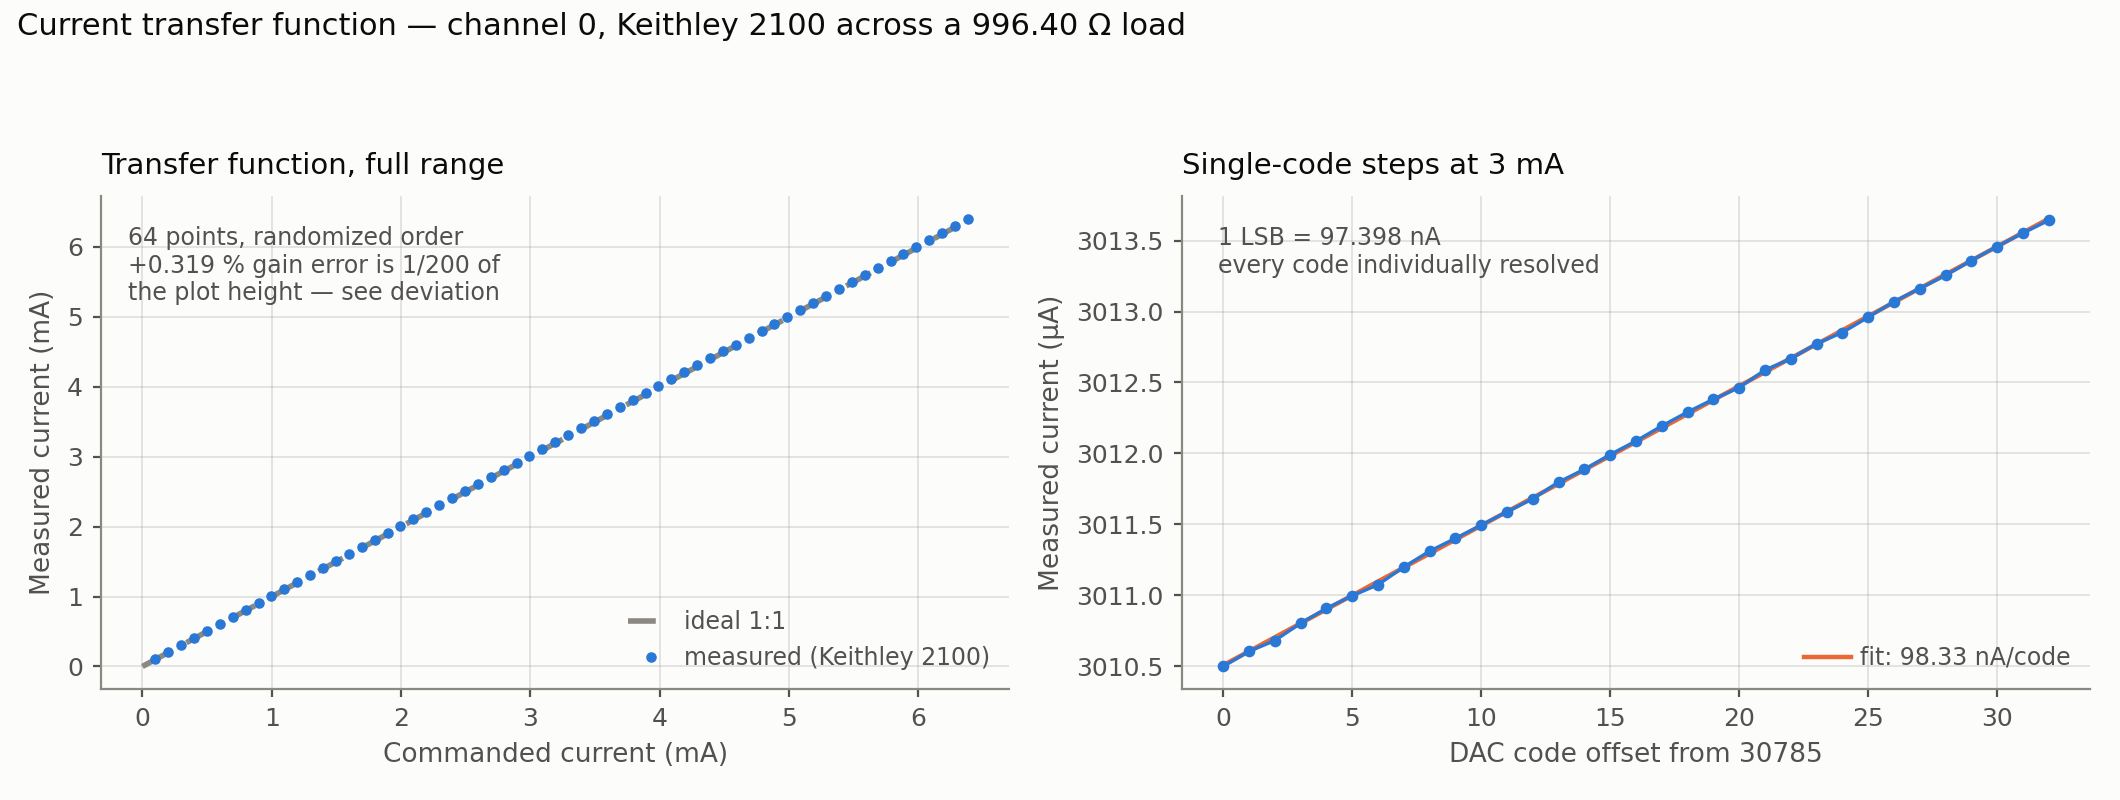
\includegraphics[width=\textwidth]{figures/i-transfer.png}
  \caption{Current transfer function, channel~0. Left: commanded current vs.\
  current measured by the external reference over the full 0--6.383\,mA range,
  64 points in randomized order; the $+0.319\,\%$ gain error is far too small to
  see at this scale, which is why the deviation plot of
  Figure~\ref{fig:i-deviation} is the informative view. Right: the single-code
  region at 3\,mA, showing that individual DAC codes ($1\,\text{LSB}=97.4$\,nA)
  are cleanly resolved by the reference.}
  \label{fig:i-transfer}
\end{figure}

% --- Current deviation: ext DMM + onboard ADC ---
\begin{figure}[htbp]
  \centering
  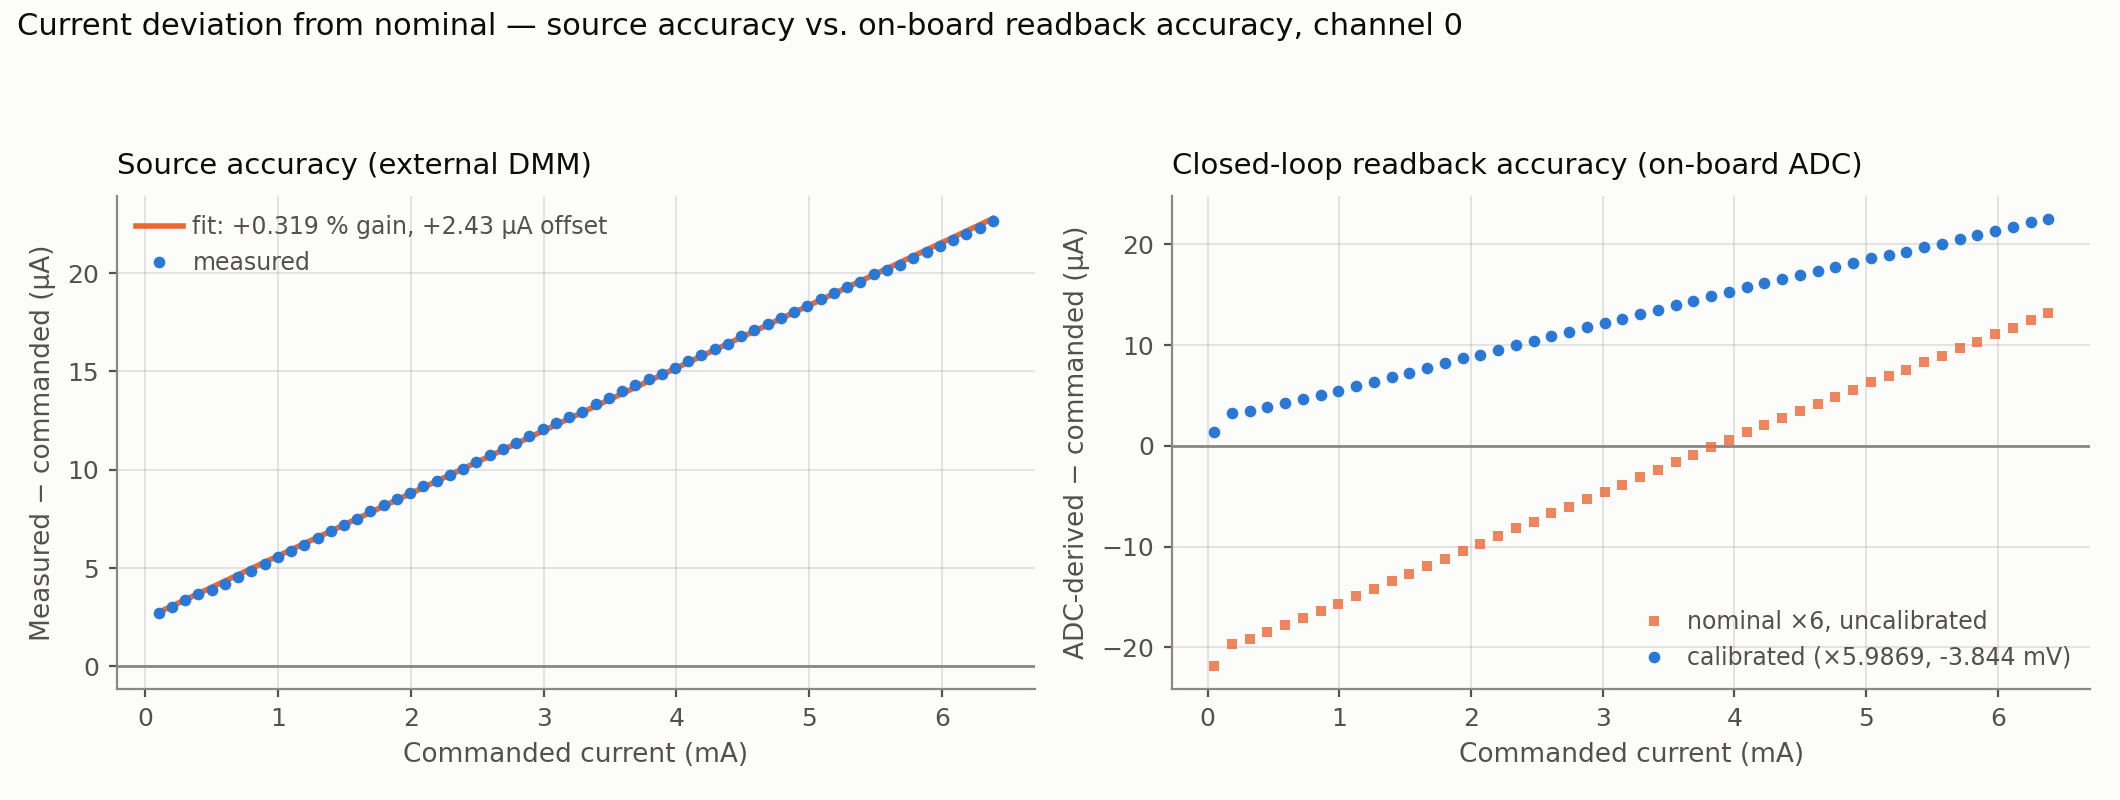
\includegraphics[width=\textwidth]{figures/i-deviation.png}
  \caption{Current deviation from nominal, channel~0. Left: against the external
  reference DMM --- source accuracy. The entire error is one straight line, i.e.\
  a gain term plus an offset, with $0.070\,\mu$A rms left over. Right: against
  the on-board AD7193 readback --- closed-loop measurement accuracy, after the
  sense-divider correction, shown both with the nominal $\times6$ divider ratio
  and after the two-parameter sense calibration of
  Section~\ref{sec:vsense-linearity}.}
  \label{fig:i-deviation}
\end{figure}

\paragraph{Code-level resolution and linearity.} Resolution was measured with
the external DMM alone --- the on-board ADC takes no part --- by stepping the
DAC one code at a time and deriving current from the voltage across the
four-wire load. The DAC is 16-bit over the 0--6.3830\,mA span, so the
instrument offers \textbf{65\,536 individually settable currents per channel},
on each of the 64 channels independently, with
\[
  1\,\text{LSB} = 97.398\,\text{nA} = 97.03\,\mu\text{V across }996.4\,\Omega .
\]
The 2100's own noise over the same reads is $\approx$8\,$\mu$V, i.e.\ $0.08$\,LSB,
so the reference resolves roughly twelve steps within a single DAC code and
\emph{every code is individually resolvable}; the DAC's LSB, not the
measurement, sets the resolution. Points taken: 64 across the full range in
randomized order, plus 33-code ($\pm16$\,LSB) sweeps centred on 1.0, 3.0 and
5.0\,mA. Because a $\pm16$-code span is short enough that the converter's own
integral nonlinearity dominates its local slope, the mean step measured that way
($98.9$\,nA) characterizes \emph{step uniformity}, not gain; the gain figure is
the full-range fit above.

\medskip
\noindent\begin{tabular}{@{}llr@{}}
\toprule
\textbf{Quantity} & \textbf{Measured} & \textbf{As \% FS} \\
\midrule
Settable levels & 65\,536 per channel (1\,LSB $=97.398$\,nA) & --- \\
INL (randomized order) & rms 0.64\,LSB, max $-1.31$\,LSB & $0.0020\,\%$ \\
INL (monotonic order) & rms 0.60\,LSB, max $-1.51$\,LSB & $0.0023\,\%$ \\
DNL & max $0.40$\,LSB & --- \\
Monotonicity & 0 non-monotonic steps in 96 & --- \\
Effective resolution & 15.6 of 16 bits & --- \\
\bottomrule
\end{tabular}
\medskip

The converter is monotonic everywhere measured, at every centre and every
settling time tried.

\paragraph{Load self-heating, and why it no longer confounds the INL.} Measuring
INL on a resistive load is not straightforward, because code order and thermal
state are confounded: a monotonic 0--6.38\,mA ramp raises dissipation from 0 to
40\,mW across the sweep, and a metal-film resistor at $\sim$50\,ppm/$^\circ$C
warming a few degrees drifts $\sim$250\,ppm --- comparable to the
$\sim$0.002\,\% FS being resolved. In an earlier configuration of this bench,
with the load convecting freely, a monotonic ramp returned an INL some 60\,\%
larger than a randomized sweep of the same converter, the difference being
entirely thermal.

The measurements reported here remove that mechanism at its source: the load is
held at ambient by forced air, so its dissipation no longer maps onto code order.
Two independent controls confirm it rather than assume it. First, the codes are
still visited in random order with a fixed reference point re-measured every
fourth point and each datum corrected by the reference interpolated to its
timestamp. Second --- and this is the decisive one --- the same 48 codes were
also swept \emph{monotonically}, the worst case for a self-heating artifact. The
two agree: \textbf{rms 0.64\,LSB randomized against 0.60\,LSB monotonic}, well
inside the 0.09\,LSB per-code repeatability. A thermal term large enough to
matter cannot survive that comparison, so the residual is genuine converter
nonlinearity.

The practical consequence for anyone reproducing this work is that randomized
order is a cheap check rather than a requirement, provided the load is
temperature-stabilized; without stabilization it is mandatory, and a monotonic
ramp will overstate INL substantially.

\begin{figure}[htbp]
  \centering
  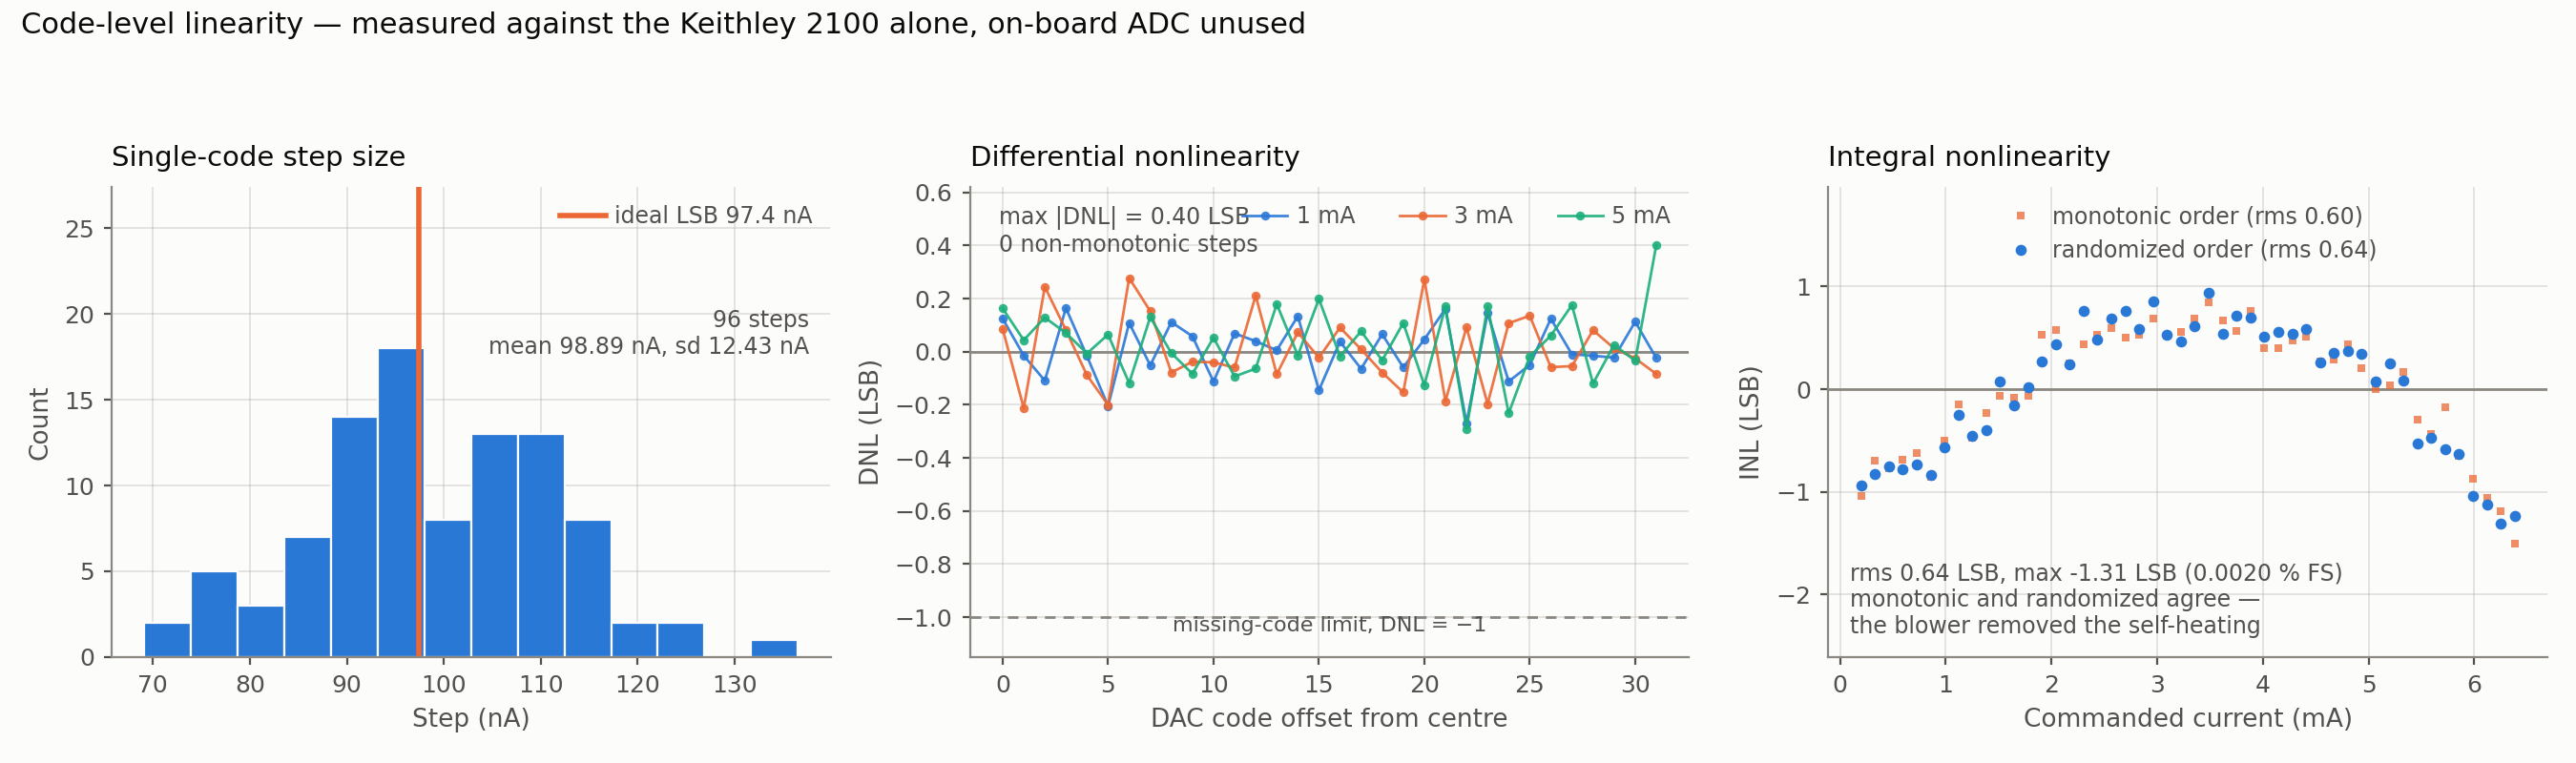
\includegraphics[width=\textwidth]{figures/i-linearity.png}
  \caption{Code-level linearity, channel~0, measured against the external DMM
  with the on-board ADC unused. Left: single-code step-size distribution
  (1\,LSB $=97.4$\,nA over the 0--6.383\,mA span). Centre: current-mode
  differential nonlinearity, max $0.40$\,LSB, with no step approaching the
  $-1$\,LSB missing-code limit at any of the three centres. Right: integral
  nonlinearity in randomized and in monotonic code order. With the load held at
  ambient by forced air the two agree (rms 0.64 vs.\ 0.60\,LSB), which is the
  evidence that load self-heating no longer contaminates the measurement.}
  \label{fig:i-linearity}
\end{figure}

% --- Precision / std dev ---
\begin{figure}[htbp]
  \centering
  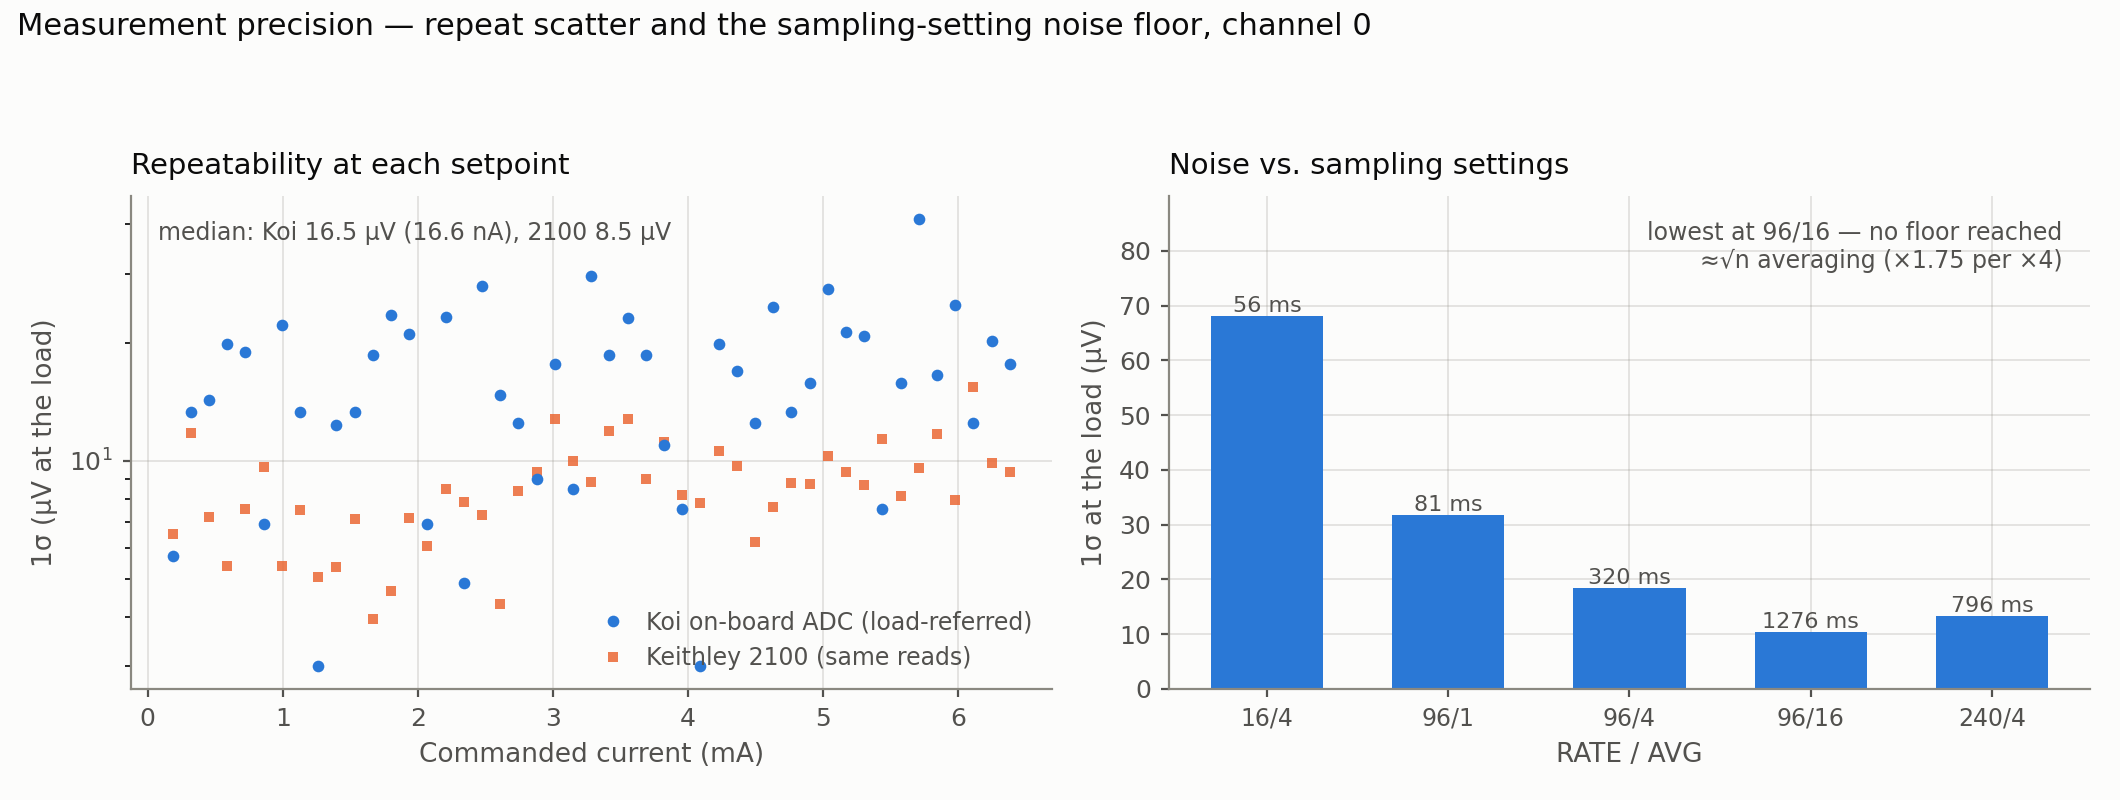
\includegraphics[width=\textwidth]{figures/i-precision.png}
  \caption{Measurement precision, channel~0. Left: $1\sigma$ over repeated reads
  at each setpoint across the operating range, for the on-board ADC
  (load-referred) and for the reference DMM over the same reads. Right: noise
  against the two sampling controls, annotated with the per-read cost. Noise
  falls monotonically as $\sqrt{n}$ with averaging over the whole range tested,
  so no floor is reached; the choice of setting is a speed/noise trade rather
  than a search for a floor (Section~\ref{sec:noise}).}
  \label{fig:i-precision}
\end{figure}

\subsection{Sense-divider correction and end-to-end resistance accuracy}
\label{sec:divider-correction}
The divider-current correction
$I_\text{heater}=I_\text{source}-V_\text{heater}/120\,\text{k}\Omega$ was
validated end-to-end by comparing the resistance the instrument reports against
the four-wire value of the reference load (996.4\,$\Omega$). Resistance is
computed from the calibrated sense model of Section~\ref{sec:vsense-linearity},
the commanded current, and the divider correction:

\medskip
\noindent\begin{tabular}{@{}lrr@{}}
\toprule
\textbf{Range} & \textbf{$R$ reported} & \textbf{vs.\ four-wire} \\
\midrule
$I\ge0.5$\,mA & $1000.65\pm0.80\,\Omega$ & $+0.426\,\%$ \\
$I\ge1.0$\,mA & $1000.44\pm0.45\,\Omega$ & $+0.406\,\%$ \\
$I\ge2.0$\,mA & $1000.27\pm0.24\,\Omega$ & $+0.389\,\%$ \\
\bottomrule
\end{tabular}
\medskip

The $+0.4\,\%$ bias is \emph{not} a failure of the divider correction: it is the
$+0.319\,\%$ drive gain error of Section~\ref{sec:current-char} propagating
through, because $R$ is computed from \emph{commanded} rather than measured
current. The quantity that characterizes the instrument is the scatter,
$\pm0.24$--$0.45\,\Omega$ ($0.02$--$0.05\,\%$), which is what remains once
\texttt{calSlope} is trimmed. Correspondingly, the resistance accuracy of an
uncalibrated unit is set by the drive scale factor, and of a calibrated unit by
the sense residual (Section~\ref{sec:vsense-linearity}) and the drive linearity
($0.0011\,\%$ FS).

\note{This measurement is a useful check on the whole analysis chain. An earlier
campaign, with the load resistance mistakenly taken as $1005.68\,\Omega$ instead
of $996.4\,\Omega$, reported $-0.372/-0.393/-0.412\,\%$ with
$\pm0.87/\pm0.49/\pm0.27\,\Omega$ scatter --- the same magnitudes and the same
scatter as above, with the sign reversed, which is exactly what a $0.92\,\%$
error in $R$ predicts. The scatter, the figure of merit here, is unchanged by
the correction, as it must be: it does not depend on $R$.}

\subsection{Voltage-sense linearity and the low-signal gain deficit}
\label{sec:vsense-linearity}

The voltage-sense path was characterized against a Keithley 2100 6.5-digit DMM
connected directly across the load. The DMM was automated over USB-TMC
(\texttt{tools/keithley2100.py}, driven by \texttt{tools/vsweep\_dmm.py}), so
each sweep point is the mean of eight readings at 10 power-line cycles.
Channel~0 was driven into a 996.4\,$\Omega$ resistor (four-wire measured)
over 0.005--3\,mA, with the ADC at \texttt{RATE}\,96, \texttt{AVG}\,4, gain~1,
SINC4, chopper off. The DMM was held on a \emph{fixed} 10\,V DC range for the
whole sweep: autoranging would split the points across two range calibrations
and fold the difference between them directly into the fitted intercept, which
is the quantity of interest here.

The transfer function is \textbf{piecewise linear}, with a knee that this sweep
brackets between $V_\text{node}=42.0$ and $46.9$\,mV --- i.e.\ $44\pm2$\,mV,
$\approx$44\,$\mu$A into this load. The incremental ratio collapses from 10.8 to
7.2 across that single step and reaches its asymptote within two more:

\medskip
\noindent\begin{tabular}{@{}rrrrr@{}}
\toprule
\textbf{$I_\text{cmd}$ (mA)} & \textbf{$V_\text{node}$ (mV)} & \textbf{$V_\text{ADC}$ (mV)} & \textbf{incr.\ ratio} & \textbf{implied offset (mV)} \\
\midrule
0.005 & 7.245   & 0.473   & ---   & $-0.737$ \\
0.010 & 12.266  & 0.888   & 12.09 & $-1.160$ \\
0.020 & 22.120  & 1.715   & 11.82 & $-1.979$ \\
0.030 & 32.066  & 2.562   & 11.64 & $-2.792$ \\
0.040 & 42.008  & 3.456   & 10.80 & $-3.559$ \\
\midrule
0.045 & 46.946  & 4.145   & \textbf{7.17} & $-3.695$ \\
0.050 & 51.839  & 4.943   & 6.13  & $-3.714$ \\
0.100 & 101.484 & 13.197  & 6.009 & $-3.750$ \\
0.200 & 200.564 & 29.707  & 6.001 & $-3.786$ \\
1.000 & 993.703 & 162.128 & 5.988 & $-3.813$ \\
2.000 & 1985.119 & 327.735 & 5.987 & $-3.765$ \\
3.000 & 2976.507 & 493.342 & 5.986 & $-3.712$ \\
\bottomrule
\end{tabular}
\medskip

Least-squares fits to the two regimes:
\[
  \underbrace{V_\text{ADC} = \frac{V_\text{node}}{11.696} - 0.165\,\text{mV}}_{\text{below the knee},\ r^2=0.9995}
  \qquad
  \underbrace{V_\text{ADC} = \frac{V_\text{node}}{5.9883} - 3.752\,\text{mV}}_{\text{above the knee},\ r^2=1.0000000}
\]

\paragraph{Interpretation.} A residual of $\approx-3.5$\,mV at the ADC pin
($\approx-21$\,mV load-referred) had previously been characterized as a fixed
additive measurement offset. This sweep shows that description is an artifact
of never sampling below 0.05\,mA: the low-current regime has an intercept of
$-0.165$\,mV, i.e.\ \emph{essentially zero offset}, and instead roughly half the
correct gain (11.70 vs.\ 5.99). The path therefore arrives at the knee already
$\approx$3.6\,mV short and thereafter tracks with the \emph{correct} slope,
which is indistinguishable from a fixed offset to any measurement taken above
the knee. The offset is a consequence of the low-signal gain deficit, not an
independent term.

Quantitatively this is consistent with a current drawn from the ADC pin that is
ohmic ($\approx$17.4\,k$\Omega$) below $\approx$3.9\,mV and saturates at
$\approx$225\,nA above it
($225\,\text{nA}\times(100\,\text{k}\Vert20\,\text{k}=16.67\,\text{k}\Omega)=3.75$\,mV)
--- the resistive-then-constant-current signature of a leaky junction or ESD
structure. Note that 225\,nA is roughly $200\times$ the AD7193's buffered
input-leakage specification, and that a power-off resistance check cannot detect
it (the divider measures a textbook 16.691\,k$\Omega$ pin-to-ground).

\paragraph{Practical consequence.} Above the knee --- i.e.\ for any load
current above $\approx$45\,$\mu$A, which covers the entire intended thermo-optic
operating range --- the sense path is linear to $r^2=1.0000000$, and what remains
after the two-parameter fit is $38.6\,\mu$V rms ($61.5\,\mu$V worst) at the ADC
pin, equivalently $368\,\mu$V node-referred or \textbf{58\,ppm of the 6.4\,V
full-scale node span}. The offset is a single additive constant that calibrates
out. Below the knee the reported voltage is \emph{not} trustworthy and should not
be used for resistance or power estimation. This bounds the usable low end of the
measurement range and is reported here as a characterized limitation.

\paragraph{On the divider ratio.} The in-situ fit returns 5.99 rather than the
6.0017 obtained by back-driving the divider with the current source removed.
The difference is not a divider error: $\approx$1.9\,$\Omega$ of series
resistance in the load path between the divider tap and the DMM connection
carries the load current, so the divider sees $V_\text{DMM}+I R_s$, a
current-proportional term that lands entirely in the fitted ratio
($6.0017/(1+R_s/996.4)=5.988$). The nominal $\times6$ of
Section~\ref{sec:description} is correct. The corollary is methodological: an
in-situ voltage-vs-voltage sweep cannot measure the true divider ratio and will
always return $\approx$5.99; ratio must come from a back-drive measurement, and
in-situ sweeps should be used for offset and linearity only.

\todo{Repeat on a second channel and a second board. The data above is one
channel on one board; the earlier per-board clustering of this residual makes a
225\,nA leak on \emph{every} channel implausible unless it is inherent to the
AD7193 input structure, which the single-channel data cannot distinguish.}
\todo{Decisive localization: probe the ADC pin directly across the same
low-current points. If the pin voltage itself shows the 11.73$\rightarrow$5.99
knee the current is drawn at the node (board/ESD leakage, fixable upstream); if
the pin tracks a clean 6:1 and only the reported code shows the knee, it is
internal to the AD7193. Attach the meter for \emph{all} points so its loading of
this unfiltered $\approx$16.7\,k$\Omega$ node stays common-mode.}

\begin{figure}[htbp]
  \centering
  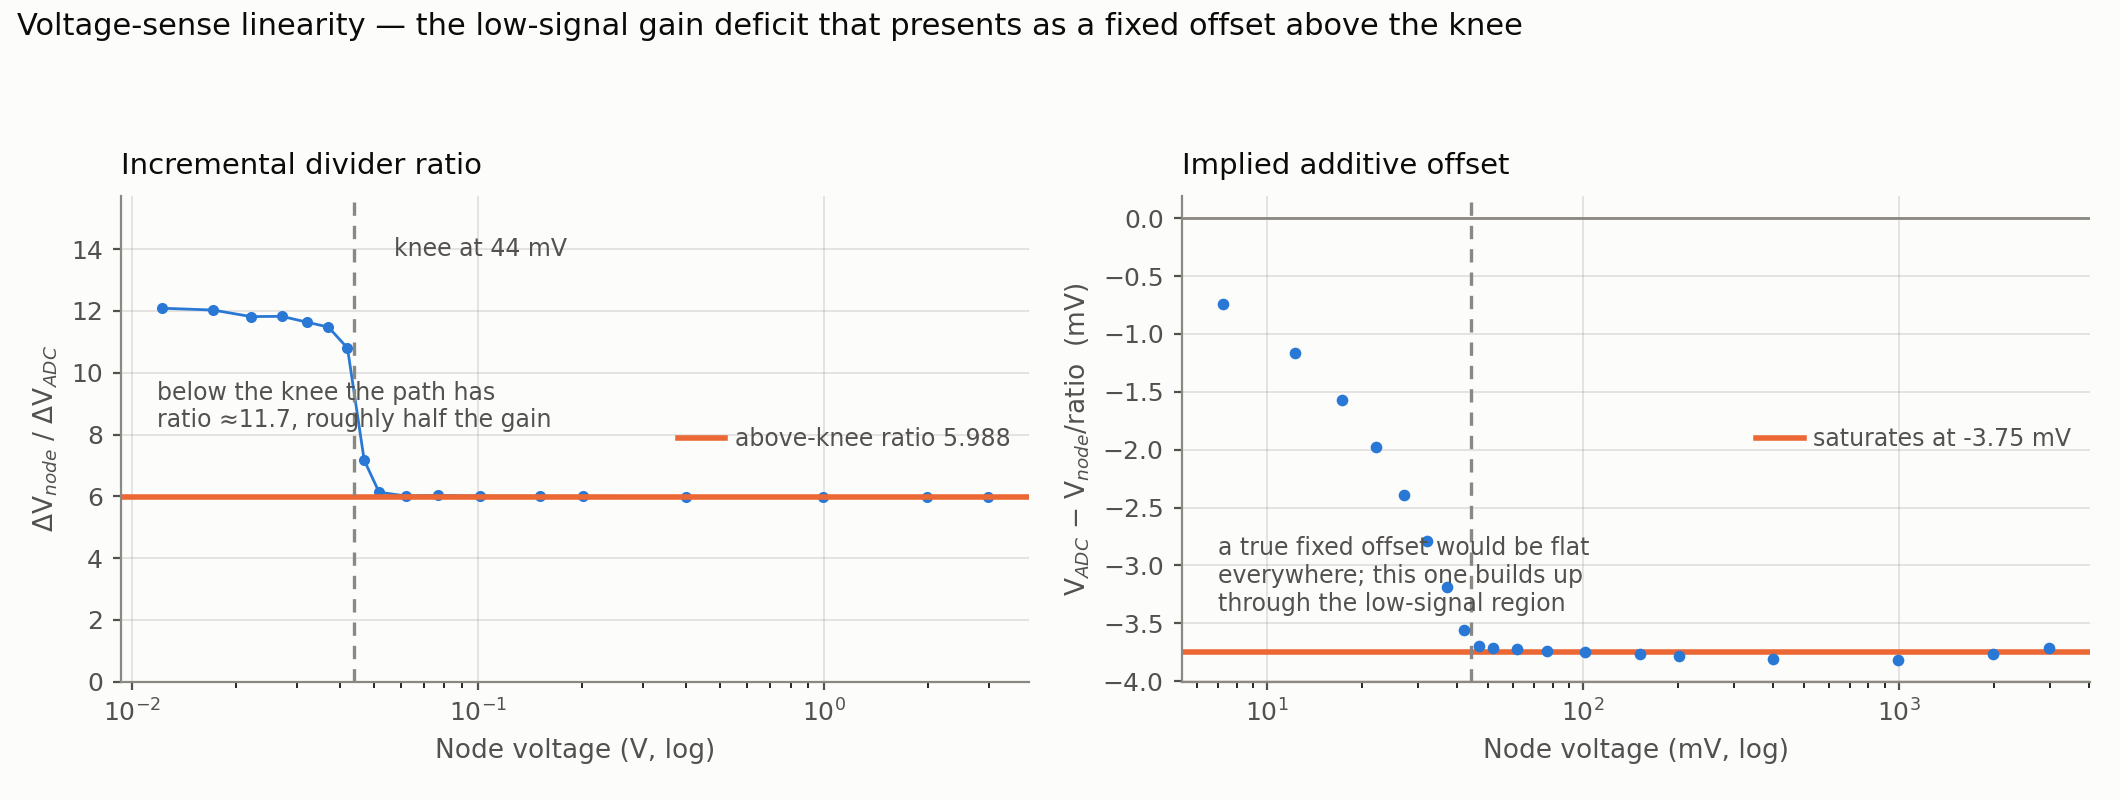
\includegraphics[width=\textwidth]{figures/v-sense.png}
  \caption{Voltage-sense linearity, channel~0. Left: the incremental divider
  ratio $\Delta V_\text{node}/\Delta V_\text{ADC}$ against node voltage, showing
  the collapse from $\approx$11.7 to the correct 5.99 at the knee
  ($V_\text{node}=44\pm2$\,mV, dashed). Right: the additive offset implied if one
  insists on describing the path with the above-knee gain --- it builds up
  through the low-signal region and saturates at $-3.75$\,mV, which is the
  signature that distinguishes a low-signal gain deficit from a true fixed
  offset. A genuine offset would be flat everywhere.}
  \label{fig:v-sense-linearity}
\end{figure}

\subsection{Noise and resolution}
\label{sec:noise}
Measurement noise was characterized by repeated single-channel reads at a fixed
commanded current (channel~0, 1.0\,mA into 996.4\,$\Omega$, 30 reads per
setting, the first five after each change discarded because conversions taken
before the filter settles are invalid), sweeping the two sampling controls: \texttt{RATE} (the AD7193 filter
word) and \texttt{AVG} (on-microcontroller averaging). The Keithley 2100's own
spread over the same reads is quoted alongside as a bound on how much of the
observed noise originates in the source and load rather than the ADC.

\medskip
\noindent\begin{tabular}{@{}rrrrrrr@{}}
\toprule
\textbf{RATE} & \textbf{AVG} & \textbf{t/read} & \textbf{1$\sigma$ at pin} & \textbf{1$\sigma$ at load} & \textbf{equiv.\ current} & \textbf{2100 1$\sigma$} \\
\midrule
8   & 4  & 29\,ms   & 30.5\,$\mu$V & 183\,$\mu$V & 184\,nA & --- \\
16  & 4  & 56\,ms   & 11.36\,$\mu$V & 68.2\,$\mu$V & 68.4\,nA & 8.82\,$\mu$V \\
96  & 1  & 81\,ms   & 5.29\,$\mu$V & 31.8\,$\mu$V & 31.9\,nA & 6.29\,$\mu$V \\
96  & 4  & 320\,ms  & 3.08\,$\mu$V & 18.5\,$\mu$V & 18.6\,nA & 10.45\,$\mu$V \\
96  & 16 & 1276\,ms & \textbf{1.72\,$\mu$V} & 10.3\,$\mu$V & 10.4\,nA & 11.94\,$\mu$V \\
240 & 4  & 796\,ms  & 2.20\,$\mu$V & 13.2\,$\mu$V & 13.3\,nA & 7.92\,$\mu$V \\
\bottomrule
\end{tabular}
\medskip

Per-read time follows $0.83\,\text{ms}\times\texttt{RATE}\times\texttt{AVG}$ at
every point measured. Noise falls monotonically across the whole grid ---
$11.36\to5.29\to3.08\to1.72\,\mu$V, a factor $1.75$ per fourfold increase in
averaging, i.e.\ essentially $\sqrt{n}$ --- so \textbf{no noise floor is reached
within the settings tested}, and these data do not establish where one lies.
Averaging is also the more efficient lever than filter length here: at $1.6\times$
the time, \texttt{RATE}\,96/\texttt{AVG}\,16 ($1276$\,ms, $1.72\,\mu$V) beats
\texttt{RATE}\,240/\texttt{AVG}\,4 ($796$\,ms, $2.20\,\mu$V). At the quietest
setting the pin-referred noise is below the reference DMM's own spread over the
same interval, so the figure quoted there is an upper bound on the instrument.

The choice of operating point is therefore a straightforward speed/noise trade
rather than a search for a floor. \texttt{RATE}\,8 / \texttt{AVG}\,4 refreshes
the whole 64-channel array in 1.7\,s at $184$\,nA equivalent noise and is the
practical setting for live monitoring; \texttt{RATE}\,96 / \texttt{AVG}\,16 is
$\sim$18$\times$ quieter for deliberate single-channel measurements.

\subsection{Thermal validation}
\label{sec:thermal}
Section~\ref{sec:description} claims the design needs no heatsinking because
the dissipation is distributed: worst case per transmitter is roughly
$(V_\text{supply}-V_\text{load})\times I \approx 120$\,mW (6\,mA into a
near-short), i.e.\ $\sim$1\,W per fully driven board spread across eight
packages --- the same distributed-dissipation approach used by commercial
multichannel drivers, so this is standard practice to be \emph{validated}, not
a novelty to be claimed. \todo{Validate: all 64 channels at maximum current
into worst-case (low-R) loads, thermal soak to steady state; report package /
board temperatures (IR camera or thermocouple), the temperature rise above
ambient, and --- the part users actually care about --- how much the warm-up
shifts the sourced current and the reference (couples to the drift and warm-up
tests in the noise section). State the derating, if any, for enclosed /
stacked operation.}

\subsection{Throughput}
\label{sec:throughput}
The continuous-conversion sequencer reads one full 8-channel board per pass
instead of issuing per-channel single conversions, so the readout is gated by
filter settling rather than by a fixed per-channel restart penalty. Measured on
a fully populated 8-board, 64-channel system:

\medskip
\noindent\begin{tabular}{@{}rrrrr@{}}
\toprule
\textbf{\texttt{RATE}} & \textbf{\texttt{AVG}} & \textbf{per board (8 ch)} & \textbf{full array (64 ch)} & \textbf{array refresh} \\
\midrule
8  & 1 & 0.064\,s & \textbf{0.46\,s} & 2.17\,Hz \\
8  & 4 & 0.224\,s & \textbf{1.74\,s} & 0.57\,Hz \\
16 & 4 & 0.436\,s & 3.43\,s & 0.29\,Hz \\
32 & 4 & 0.860\,s & 6.82\,s & 0.15\,Hz \\
\bottomrule
\end{tabular}
\medskip

All 64 channels returned valid data at every setting. Per-board time
$\times\,8$ reproduces the full-array time to within 2\,\% throughout, which
confirms there is no significant fixed per-board overhead: the scan cost is
settling, and it scales exactly as
$0.83\,\text{ms}\times\texttt{RATE}\times\texttt{AVG}$ per channel.

Two practical notes. The host-side command deadline is 10\,s, so whole-array
reads above $\approx$\texttt{RATE}\,48 at \texttt{AVG}\,4 exceed it and must be
issued per board --- which is what the host GUI does in normal operation.
Second, the readout is not yet optimized: the SPI clock is 1\,MHz and the
per-board scans are sequential, so overlapping them or raising the clock is
available headroom, not a claimed result.

\subsection{Channel-to-channel crosstalk and board reproducibility}
\todo{Quantify crosstalk between adjacent channels and consistency across the
8 daughterboards.}

\begin{figure}[htbp]
  \centering
  \plotph{0.46\textwidth}{4.4cm}{CURRENT-MODE CROSSTALK\\(aggressor ch1--7 vs.\ victim ch0)}\hfill
  \plotph{0.46\textwidth}{4.4cm}{CURRENT-MODE POWER INTO LOAD\\(power vs.\ current, per load R)}
  \caption{Left: current-mode crosstalk --- shift in a victim channel's current
  as the other seven channels are swept across their range. Right: power
  delivered to representative loads vs.\ commanded current, with the nominal
  maximum-power point marked.}
  \label{fig:i-crosstalk-power}
\end{figure}

% =====================================================================
\section{Capabilities and use cases}
\label{sec:capabilities}
\todo{Demonstration: drive an array of TiN heaters on a photonic chip, measure
$R$ vs.\ power, show phase tuning / a programmed mesh state. This demo is what
backs the closed-loop-tuning claim in the abstract and Section~1 --- it is
required, not optional, and is deliberately scheduled \emph{last}: it depends
on first resolving the offset-current anomaly and tightening the measurement
chain (Section~\ref{sec:validation}). State limitations: 0--6\,mA range,
sub-100\,$\mu$A unreliable, write-only DAC bus, etc.}

% =====================================================================
\section*{Declarations}
\todo{CRediT author contributions, conflict-of-interest statement, funding,
data/code availability (Zenodo DOI), acknowledgements.}

\bibliographystyle{plain}
\bibliography{refs}

\end{document}
